\documentclass{VUMIFPSkursinis}
\usepackage{algorithmicx}
\usepackage{algorithm}
\usepackage{algpseudocode}
\usepackage{amsfonts}
\usepackage{amsmath}
\usepackage{bm}
\usepackage{caption}
\usepackage{color}
\usepackage{float}
\usepackage{graphicx}
\usepackage{listings}
\usepackage{subfig}
\usepackage{wrapfig}
\usepackage{longtable}

\usepackage{enumitem}
%PAKEISTA, tarpai tarp sąrašo elementų
\setitemize{noitemsep,topsep=0pt,parsep=0pt,partopsep=0pt}
\setenumerate{noitemsep,topsep=0pt,parsep=0pt,partopsep=0pt}

% Titulinio aprašas
\university{Vilniaus universitetas}
\faculty{Matematikos ir informatikos fakultetas}
\department{Programų sistemų bakalauro studijų programa}
\papertype{Projektinis darbas}
\title{Paieškos proceso ir jos rezultatų pateikimo vartotojams panaudojamumas VUL Santaros klinikų tinklalapyje}
\titleineng{The Usability of the Search Process and Presenting its Results to the User for VUH Santaros klinikos website}
\status{4 kurso 3 grupės studentas}
\author{Tomas Kiziela}
% \secondauthor{Vardonis Pavardonis}   % Pridėti antrą autorių
\supervisor{doc. Kristina Lapin}
\date{Vilnius – \the\year}

% Nustatymai
% \setmainfont{Palemonas}   % Pakeisti teksto šriftą į Palemonas (turi būti įdiegtas sistemoje)
\bibliography{bibliografija}

\begin{document}
	
% PAKEISTA	
\maketitle
\cleardoublepage\pagenumbering{arabic}
\setcounter{page}{2}

%TURINYS
\tableofcontents



\sectionnonum{Įvadas}
Šiame darbe tyrinėjami praktiniai sprendimai Vilniaus Universiteto Ligoninės (VUL) Santaros klinikų tinklapio santa.lt panaudojamumo problemoms spręsti. Darbe surasti reikalavimai sistemai kylantys iš naudotų poreikių ir panaudojamumo analizės, architektūriniai sprendimai ir technologijos atitinkančios reikalavimus. Šis darbas yra autoriaus kursinio darbo tesinys \cite{Kursinis}.

Autoriaus kursiniame darbe rasta, kad santa.lt tinklapio naudotojams yra aktualu rasti registraciją pas gydytoją ir ligoninės kontaktus, tačiau tinklapyje tai padaryti užtrunka ilgiau nei turėtų. Be šių problemų tinklapyje yra ir kitų panaudojamumo problemų rastų per panaudojamumo analizę. Tinklapio paieškos rezultatai neatitinka naudotojo įvestos užklausos, yra prastai surūšiuoti, filtravimas nėra efektyvus ir nėra patarimų kaip reikėtų teisingai naudoti paieškos sistemą. Navigacijos sistema turi per daug lygių ir yra nepakankamai plati, kategorijų pavadinimai neatitinka informacijos viduje ir puslapio elementai neteikia pakankamo atsako naudotojo veiksmams. Šiuos ir kitus rastus trūkumus ketinama ištaisyti galutinėje sistemoje.

Lietuva pagal 2018 metų DESI indeksą įvertinta 94 balais pagal plačiajuosčio ryšio kainą, 3 vieta Europos Sąjungoje (ES), o naujienas internetu skaito net 93\% gyventojų, daugiau nei bet kurioje kitoje ES valstybėje\cite{InternetasLt}. Iš to matosi, kad lietuviai turi prieinamą internetą ir dažnai jį pasitelkia kaip informacijos šaltinį. Technologiškai pažengusiose valstybėse su gerai išvystyta interneto infrastruktūra gyventojai dažnai ieško informacijos apie sveikatą internetu\cite{InternetUseByPublicSAEn}\cite{InternetUseByPublicHKEn}, tikėtina, kad tai galioja ir Lietuvoje.

VUL Santaros klinikos yra viena didžiausių Lietuvos ligoninių. Joje dirba virš 5000 darbuotojų ir kasmet gydoma apie milijonas pacientų\cite{VulSkApieMusLt}. Atrodo natūralu daryti prielaidą, kad nemažai pacientų ir lankytojų apie ligoninę domisi internetu ir ligoninei yra svarbu turėti tinklapį atitinkantį naudotojų lūkesčius.

Šio \textbf{darbo tikslas} yra apibrėžti reikalavimus, suprojektuoti galutinę sistemą ir pasirinkti technologijas tinkančias sistemos kūrimui. 

Uždaviniai:
\begin{enumerate}
	\item Identifikuoti reikalavimus sistemai
	\item Suprojektuoti tinklapį
	\item Palyginti ir pasirinkti technologijas reikalingas tinklapio įgyvendinimui
\end{enumerate}

\sectionnonum{Panaudojamumo analizės rezultatai}
Kursiniame darbe buvo įvertintas esamo tinklapio panaudojamumas pagal David Travis gaires ir Jakob Nielsen euristikas\cite{Kursinis}. Prie defektų parašyti skaičiai nurodo kuris maketas (pav.) ir kuri maketo dalis (d.) juos taiso.

\begin{center}
\captionof{table}{Paieškos panaudojamumo gairių vertinimas pradiniam puslapiui}
\begin{tabular}{ |p{13cm}|p{2,5cm}| } 
 \hline
	Gairė & Ar tenkina? \\ \hline
	1) Pagrindinė paieška lengvai valdoma & tenkina \\ \hline
	2) Paieškos rezultatų puslapis naudotojui rodo, ko buvo ieškota, ir yra lengva pakeisti ir pakartoti užklausą & tenkina \\ \hline
	3) Paieškos rezultatai yra aiškūs, naudingi ir reitinguojami pagal atitikimą užklausai & ne (\ref{img:PaieškosPrototipas} pav. 2 d.) \\ \hline
	4) Paieškos rezultatų puslapis aiškiai parodo kiek rezultatų gražinta ir rezultatų skaičius per puslapį gali būti reguliuojamas naudotojo & tenkina \\ \hline
	5) Jei negražinamas nei vienas rezultatas, sistema pasiūlo idėjų ar nustatymų pagerinti užklausai atsižvelgiant į atpažįstamas įvesties problemas & ne (\ref{img:PaieškosPrototipas} pav. 4 d.) \\ \hline
	6) Paieška dailiai susitvarko su tuščia užklausa & tenkina \\ \hline
	7) Dažniausios užklausos gražina naudingus rezultatus & ne (\ref{img:PaieškosPrototipas} pav. 2 d.) \\ \hline
	8) Paieškos sistema turi šabloną arba patarimus kaip ją deramai naudoti & ne (\ref{img:PaieškosPrototipas} pav. 4 d.) \\ \hline
	9) Puslapis turi pajėgesnę paieškos sąsają leidžiančią naudotojams patikslinti užklausas & tenkina \\ \hline
	10) Paieškos rezultatų puslapis nerodo besikartojančių rezultatų & tenkina \\ \hline
	11) Paieškos laukas pakankamai ilgas dažniausių užklausų ilgiams & ne (\ref{img:PaieškosPrototipas} pav. 1 d.) \\ \hline
	12) Paieška apima visą interneto svetainę, o ne tik jos dalį & tenkina \\ \hline
	13) Jei svetainė leidžia naudotojams sudaryti sudėtingą paiešką, šios paieškos gali būti išsaugojamos ir kartojamos reguliariai & tenkina \\ \hline
	14) Paieškos sąsaja padėta, naudotojams įprastoje vietoje (viršuje dešinėje) & tenkina \\ \hline
	15) Paieškos laukas ir jo kontrolės aiškiai pavadintos & tenkina \\ \hline
	16) Puslapis palaiko paieškos strategiją ir naršymo strategiją & ne (\ref{img:PaieškosPrototipas} pav.) \\ \hline
	17) Paieškos sritis aiškiai parašyta paieškos rezultatų puslapyje ir naudotojai gali ją susiaurinti & tenkina \\ \hline
	18) Paieškos rezultatų puslapis atvaizduoja naudingą meta informaciją (informacija apie informaciją), kaip dokumento dydis, dokumento sukūrimo data ir failo tipas & tenkina \\ \hline
	19) Paieškos sistema automatiškai patikrina rašybą ir ieško daugiaskaitinių formų ir sinonimų & ne \\ \hline
	20) Paieškos sistema leidžia ieškoti panašių rezultatų („daugiau tokių“) & ne (\ref{img:PaieškosPrototipas} pav. 5 d.) \\ \hline
\end{tabular}
\label{PaieškosLentelėPrad}
\end{center}
\pagebreak


\captionof{table}{Navigacijos ir informacijos architektūros panaudojamumo gairių vertinimas}
\begin{longtable}{ |p{12,6cm}|p{2,9cm}| } 
 \hline
	Gairė & Ar tenkina? \\ \hline
	1) Yra patogus ir akivaizdus būdas judėti tarp susijusių puslapių ir skyrių ir yra lengva grįžti į pagrindinį puslapį & tenkina \\ \hline
	2) Informacija, kurios naudotojams dažnai prireikia yra lengvai pasiekiama iš daugumos puslapių & tenkina \\ \hline
	3) Navigacijos pasirinkimai išrikiuoti pačiu racionaliausiu arba užduočiai orientuotu būdu & tenkina \\ \hline
	4) Navigacijos sistema plati ir sekli (daug meniu elementų), o ne gili (daug meniu lygių)  & ne (\ref{img:NavigacijosPrototipas} pav. 4, 6 d.) \\ \hline
	5) Paprasta, aiškaus modelio svetainės struktūra be nereikalingų lygių & ne (\ref{img:NavigacijosPrototipas} pav. 4, 6 d.) \\ \hline
	6) Pagrindiniai puslapio skyriai pasiekiami iš bet kurio puslapio ir nėra aklaviečių & tenkina \\ \hline
	7) Navigacijos skirtukai patalpinti puslapio viršuje ir atrodo kaip paspaudžiamos versijos realaus pasaulio skirtukų & ne \\ \hline
	8) Yra svetainės žemėlapis, kuris suteikia svetainės turinio apžvalgą & tenkina \\ \hline
	9) Svetainės žemėlapį galima pasiekti iš bet kurio puslapio & tenkina \\ \hline
	10) Svetainės žemėlapis suteikia glaustą svetainės apžvalgą, o ne pernaudotą navigacijos meniu ar sąrašą kiekvienos temos & ne \\ \hline
	11) Suteikiamas geras navigacijos grįžtamasis ryšys (rodoma, kur randiesi puslapyje) & tenkina \\ \hline
	12) Kategorijų pavadinimai tiksliai apibūdina informaciją viduje & ne (\ref{img:NavigacijosPrototipas} pav. 4, 6 d.) \\ \hline
	13) Nuorodos ir navigacijos pavadinimai susidaro iš raktinių žodžių, kurių naudotojai ieškos bandydami atlikti užduotį & tenkina \\ \hline
	14) Terminologija ir susitarimai (kaip nuorodų spalvos) (maždaug) atitinka bendrą interneto naudojimą & tenkina \\ \hline
	15) Nuorodos atrodo taip pačiai skirtingose svetainės dalyse & tenkina \\ \hline
	16) Navigacijos elementams ir hiperteksto nuorodoms naudojami terminai yra nedviprasmiški ir be žargono & tenkina \\ \hline
	17) Matomi pasikeitimai, kai naudotojas užveda kursorių ant kažko paspaudžiamo (neįskaitant kursoriaus pasikeitimų) & ne (\ref{img:NavigacijosPrototipas} pav. 4, 6 d.) \\ \hline
	18) Svarbus turinys pasiekiamas iš daugiau nei vienos nuorodos (naudotojams gali reikėt skirtingų nuorodų pavadinimų) & tenkina \\ \hline
	19) Puslapiai skirti tik navigacijai (pavyzdžiui pradinis puslapis) gali būti peržiūrimi be slinkimo & tenkina \\ \hline
	20) Svetainė leidžia naudotojui kontroliuoti sąveikos greitį ir eiliškumą & tenkina \\ \hline
	21) Visuose puslapiuose yra aiškiai pažymėti išėjimai leidžiantys naudotojui pabėgti iš esamos užduoties be papildomo dialogo & tenkina \\ \hline
	22) Svetainė neišjungia naršyklės „atgal“ mygtuko ir „atgal“ mygtukas visada matomas naršyklės įrankių juostoje & tenkina \\ \hline
	23) Paspaudus „atgal“ mygtuką naudotojas visada gražinamas į puslapį, iš kurio atėjo & tenkina \\ \hline
	24) Jeigu puslapis sukuria naujus langus, jie neklaidina naudotojo (jie dialogo lango dydžio ir lengvai uždaromi) & tenkina \\ \hline
	25) Meniu instrukcijos, nurodymai ir žinutės atsiranda toje pačioje vietoje visuose puslapiuose & tenkina \\ \hline
\end{longtable}
\label{NavigacijosirIALentelėPrad}
\addtocounter{table}{-1}
\setlength{\parindent}{1cm}

\begin{center}
\captionof{table}{Euristinis vertinimas, DS - defekto sunkumas}
\begin{tabular}{ | p{3,6cm} | p{0,3cm} | p{11,6cm} | } 
 \hline
	Euristika & DS & Komentaras \\ \hline
	1) Sistemos būsenos matomumas & 2 & Paspaudus mygtuką „ieškoti“ rodomas tuščias puslapis iki paieškos rezultatų gavimo. Paieška užtrunka apie 3 sekundes, taigi galėtų būti tekstas, animacija ar progreso juosta pranešanti, kad vyksta paieška. Užvedus kursorių ant paspaudžiamų elementų kaip nuorodų ir tam tikrų elementų, šie nepasikeičia, taigi vartotojui sunkiau juos pastebėti. \\ \hline
	2) Atitikimas realiam pasauliui  & 2 & Daugumai vartotojų aktuali registracija pas gydytoją, taigi ji turėtų būti dar lengviau surandama naršant arba ieškant. (\ref{img:NavigacijosPrototipas} pav. 2 d.) \\ \hline
	3) Naudotojo valdomas dialogas & 1 & Dalis puslapių nerodo nukeliauto kelio, kai šie randami per paiešką. (\ref{img:NavigacijosPrototipas} pav. 3 d.) \\ \hline
	4) Darna ir standartai & 1 & Kai kuriuose puslapiuose pranyksta navigacijos elementai. \\ \hline
	5) Klaidų prevencija & 2 & Netinkami numatytieji nustatymai lemia, kad naudotojai dažnai atlieka netinkamą paiešką. Nėra patarimų kaip naudotis paieškos sistema. Vedant užklausą nepasiūlomi paieškos variantai. (\ref{img:PaieškosPrototipas} pav. 2, 4 d.) \\ \hline
	6) Atpažinimas geriau nei atsiminimas & 2 & Navigacija nerodo gilesnių lygių, kol neatidaromas to lygio puslapis, taigi reikia žinoti, kurioje kategorije ieškomas elementas. Trūksta vaizdų, kurie asocijuojasi su mygtukais. Nėra pagalbos naudotis tinklapiu. (\ref{img:NavigacijosPrototipas} pav. 6, 5, 1 d.) \\ \hline
	7) Naudojimo lankstumas ir našumas & 2 & Nerodomi susiję puslapiai. Negalima nueiti į giliausią kategorijos lygį vienu paspaudimu, reikia eiti per tėvinius elementus. (\ref{img:NavigacijosPrototipas} pav. 6 d.) \\ \hline
	8) Estetiškas ir minimalistinis dizainas & 2 & Pertekliniai paspaudimai bandant naviguoti per kategorijas. (\ref{img:NavigacijosPrototipas} pav. 6 d.) \\ \hline
	9) Remti klaidų atpažinimą, jų priežasčių nustatymą ir taisymą & 0 &  \\ \hline
	10) Parama ir dokumentacija & 2 & Nėra informacijos ar pavyzdžių kaip naudoti sudėtingas paieškos funkcijas. (\ref{img:PaieškosPrototipas} pav. 4 d.) \\ \hline
\end{tabular}
\label{EuristikųLentelėPrad}
\end{center}

\sectionnonum{Sprendimo maketai}
Kursiniame darbe gauti maketai nurodantys pakeitimus paieškos sistemai ir informacijos architektūrai.

\begin{figure}[H]
    \centering
    \includegraphics[scale=0.65]{img/PaieškosPrototipas}
    \caption{Paieškos sistemos maketas su pataisymais}
    \label{img:PaieškosPrototipas}
\end{figure}

\begin{figure}[H]
    \centering
    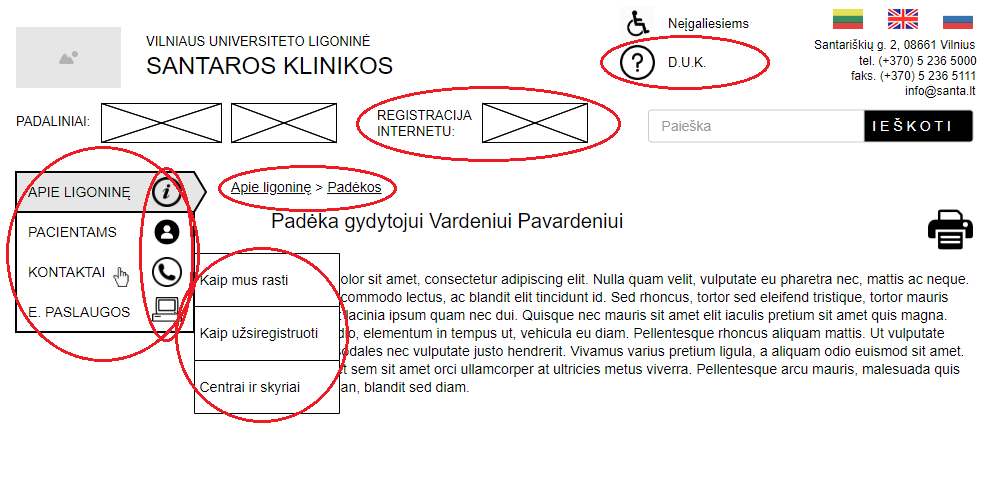
\includegraphics[scale=0.65]{img/NavigacijosPrototipas}
    \caption{Navigacijos sistemos maketas su pataisymais}
    \label{img:NavigacijosPrototipas}
\end{figure}

\section{Reikalavimų analizė}
Siekiant ištaisyti defektus informacijos architektūroje reikia apibrėžti reikalavimus, kurie išspręstų defektų priežastis. Tuo tikslu surašyti funkciniai ir nefunkciniai reikalavimai paieškos sistemai ir navigacijos ir informacijos architektūrai. Reikalavimai remiasi naudotojų poreikiais, gairėmis ir euristikomis, kurios buvo naudotos defektams surasti (lentelės \ref{PaieškosLentelėPrad}, \ref{NavigacijosirIALentelėPrad} ir \ref{EuristikųLentelėPrad}).

\subsection{Funkciniai reikalavimai paieškos sistemai}
\begin{enumerate}
	\item Pagrindinė paieška turi būti sudaryta tik iš vieno įvedimo lauko ir mygtuko, operuojama pele arba klaviatūra
	\item Paieškos rezultatų puslapis turi parodyti, atliktos užklausos įvestį ir nustatymus, jie turi būti užrašyti puslapio adrese
	\item Paieškos rezultatai turi turėti puslapio pavadinimą ir ištrauką teksto, kuri atitinką užklausą
	\item Paieškos rezultatai turi būti reitinguojami pagal atitikimą užklausai
	\item Paieškos rezultatų puslapis turi parodyti, kiek rezultatų gražinta, ir turi leisti nustatyti kiek rezultatų parodyti per puslapį
	\item Paieškos rezultatų puslapis turi leisti nustatyti kaip tiksliai rezultatai turi atitikti užklausos įvestį
	\item Paieškos rezultatų puslapis turi leisti rūšiuoti rezultatus pagal populiarumą, datą, abėcėlinę tvarką ir kategoriją
	\item Paieškos rezultatų puslapis turi leisti filtruoti pagal kategoriją
	\item Paieškos sistema turi automatiškai patikrinti rašybą, ieškoti daugiaskaitinių formų ir sinonimų
	\item Jei paieška negražina rezultatų, turi būti pasiūlomi pakeitimai užklausai pagerinti
	\item Įvedus tuščią užklausą atsidaro paieškos rezultatų puslapis be rezultatų
	\item Paieškos sistemos nustatymai pritaikyti dažnoms užklausoms
	\item Paieškos rezultatų puslapyje turi būti patarimai, kaip naudoti paiešką
	\item Paieškos rezultatų puslapis turi nerodyti pasikartojančių rezultatų
	\item Paieška turi apimti visą tinklapio turinį
	\item Nukopijavus atliktos paieškos rezultatų puslapio adresą turi būti galima kartoti paiešką
	\item Paieškos rezultatų puslapis turi parodyti naudingą informaciją apie informaciją, kaip dokumento dydis, dokumento sukūrimo data ir failo tipas
	\item Kai paieška užtrunka ilgiau nei sekundę, turi būti parodomi ženklai, kad vyksta paieškos procesas
\end{enumerate}

\subsection{Nefunkciniai reikalavimai paieškos sistemai}
\begin{enumerate}
	\item Paieškos laukas turi leisti įvesti bent 64 simbolių ilgio užklausą
	\item Paieškos laukas turi būti viršuje dešinėje
\end{enumerate}

\subsection{Funkciniai reikalavimai navigacijos ir informacijos architektūrai}
\begin{enumerate}
	\item Turi būti navigacijos sistema leidžianti pasiekti visus puslapius
	\item Navigacija turi leisti peržiūrėti visus jos elementus neatidarant kito puslapio
	\item Internetinė registracija pas gydytoją (nuoroda į sergu.lt) turi būti pasiekiama iš bet kurio puslapio
	\item Turi būti tinklapio žemėlapis, kuriame matyti tinklapio turinio apžvalga
	\item Turi būti dažnai užduodamų klausimų puslapis, kuriame paaiškinama kaip naudotis tinklapiu
	\item Turi būti režimas neįgaliesiems, leidžiantis padidinti teksto šriftą, pakeisti puslapio spalvas prastai matantiems
	\item Visuose puslapiuose, išskyrus pagrindinį, turi būti rodomas nukeliautas kelias per paryškintus navigacijos meniu skyrius ir nuorodas į tėvinius skyrius
	\item Turi būti matomi spalvos arba formos pasikeitimai, kai naudotojas užveda kursorių and kažko paspaudžiamo (ne tik kursoriaus pasikeitimai)
\end{enumerate}

\subsection{Nefunkciniai reikalavimai navigacijos ir informacijos architektūrai}
\begin{enumerate}
	\item Nuoroda į pagrindinį puslapį turi būti puslapio viršuje
	\item Nuolatiniai puslapiai sudėti į navigacijos meniu, nuoroda registracijai pas gydytoją internetu puslapio viršuje
	\item Navigacijos skyriai išrikiuoti pagal naudojimo dažnį, bet taip kad svarbūs skyriai išliktų netoli viršaus
	\item Navigacijos tėviniai skyriai turi būti susieti su paveiksliukais
	\item Navigacijos sistema turi būti plati ir sekli (daug meniu elementų), o ne gili (daug meniu lygių)
	\item Navigacijos meniu turi būti matomas visuose puslapiuose
	\item Navigacijos skirtukai turi atrodyti paspaudžiami
	\item Tinklapio žemėlapį turi būti galima pasiekti iš bet kurio puslapio
	\item Tinklapio žemėlapis turi suteikti glaustą tinklapio apžvalgą
	\item Kategorijų pavadinimai turi tiksliai apibūdinti informaciją viduje
	\item Nuorodos ir navigacijos pavadinimai turi susidaryti iš raktinių žodžių, kurių naudotojai ieškos bandydami atlikti užduotį
	\item Terminologija ir susitarimai (kaip nuorodų spalvos) turi atitikti bendrą interneto naudojimą
	\item Tekste yra nuorodos į susijusius skyrius (gali būti skirtingi nuorodų pavadinimai)
	\item Visuose puslapiuose galima grįžti atgal paspaudus naršyklės „atgal“ mygtuką
	\item Kai puslapis sukuria naujus langus, jie turi būti nedideli ir lengvai uždaromi
\end{enumerate}

\subsection{Papildomas nefunkcinis reikalavimas}
Autorius pastebėjo, kad sistema lėtai atidarinėja puslapius ir atlieka paieškas, šie veiksmai užtrunka arti 3 sekundžių. Šis sistemos bruožas labai gadina naudotojo patirtį ir turėtų būti sumažintas iki 1 sekundės ar mažiau tam, kad sistema nevargintų naudotojo.


\section{Projektavimas}
\subsection{Puslapio architektūra}
Puslapio architektūra apibūdinta kaip puslapio elementų išdėstymo sprendimai. Tinklapyje autorius rado tris pagrindinius puslapių tipus: pagrindinis puslapis, turinio puslapis ir paieškos puslapis. Pagrindinio puslapio dabartinis meniu yra nestandartinio pavidalo ir gali klaidinti naudotojus, todėl vietoj jo palikta vieta populiariems puslapiams ir kairėje įdėtas standartinis meniu. Turinio ir paieškos puslapių elementų dabartinis išdėstymas autoriui atrodo logiškas ir jo keisti nebūtina. Elementų išdėstymo schemos kiekvienam puslapio tipui pavaizduoti \ref{img:PagrindinisArch}, \ref{img:TurinysArch} ir \ref{img:PaieškaArch} paveiksluose, schemos sudarytos pagal puslapius pavaizuotus \ref{img:PagrindinisPuslapis}, \ref{img:TurinysPuslapis} ir \ref{img:PaieškaPuslapis} paveiksluose. Pagrindinio puslapio centre esantis elementas su slankiojančiais pranešimais pavadintas fasadu. Paieška yra naudotojams įprastoje vietoje (1.1.14 reikalavimas). Navigacija pagrindiniame puslapyje yra virš raukšlės (angliškai „above the fold“), kur į ją atkreips dėmesį daug daugiau vartotojų \cite{Scrolling}. Navigacija visuose kituose puslapiuose kairėje pusėje, tai gerai matoma vieta \cite{AttentionLeft} ir neužima brangios vietos viršuje.

%Pareguliuoti paveikslu dydi
\begin{figure}[htb]
    \centering
    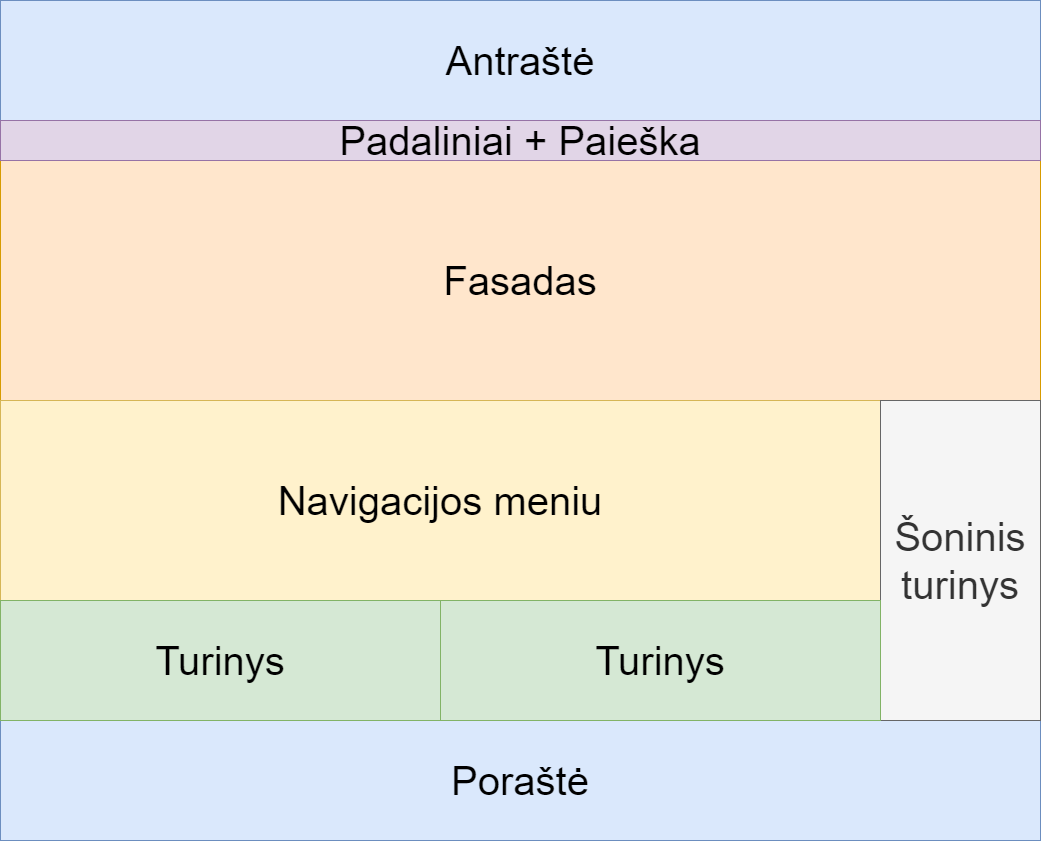
\includegraphics[scale=0.25]{img/PuslapioArchPagrindinis}
    \caption{Pagrindinio puslapio išdėstymas}
    \label{img:PagrindinisArch}
\end{figure}

\begin{figure}[htb]
\centering
\begin{minipage}{.5\textwidth}
  \centering
  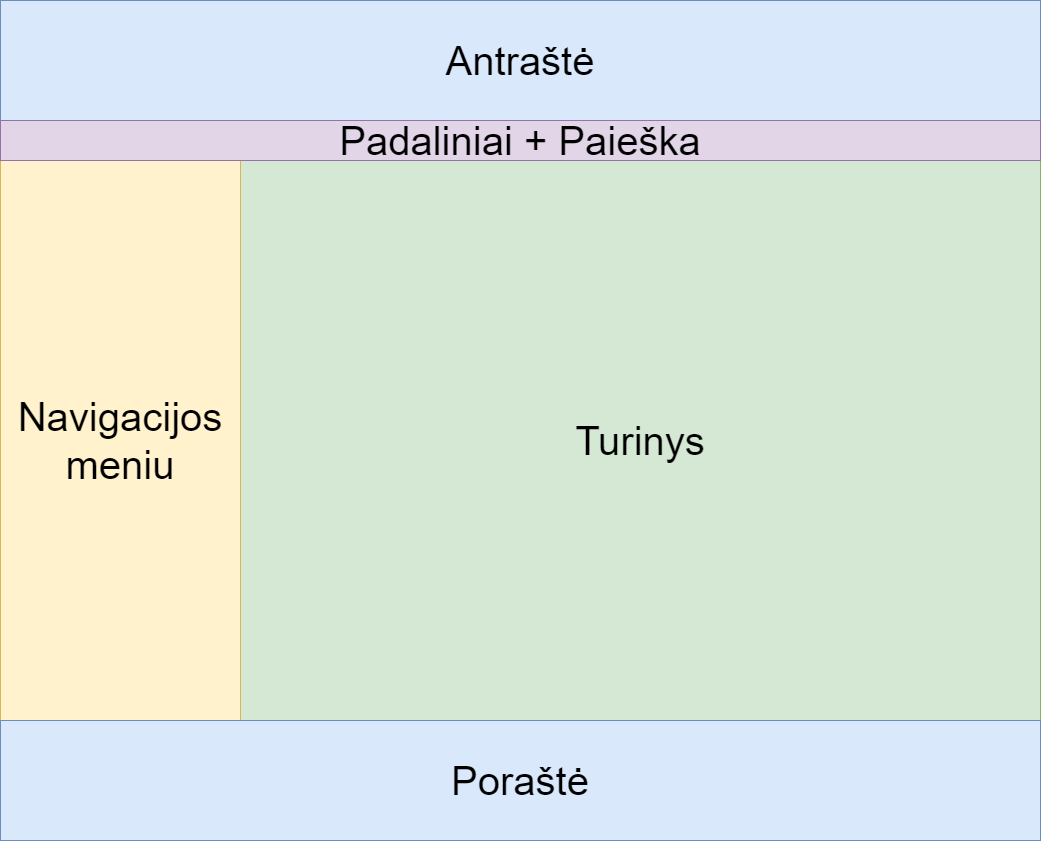
\includegraphics[width=0.9\linewidth]{img/PuslapioArchTurinys}
  \captionof{figure}{Turinio puslapio išdėstymas}
  \label{img:TurinysArch}
\end{minipage}%
\begin{minipage}{.5\textwidth}
  \centering
  \includegraphics[width=0.9\linewidth]{img/PuslapioArchPaieška}
  \captionof{figure}{Paieškos puslapio išdėstymas}
  \label{img:PaieškaArch}
\end{minipage}
\end{figure}

\subsection{Navigacijos meniu}
Tiriant navigacijos ir informacijos architektūros panaudojamumą buvo rasta, kad navigacija per daug gili (\ref{NavigacijosirIALentelėPrad}.4 defektas), yra pernelyg sudėtinga (\ref{NavigacijosirIALentelėPrad}.5 defektas) ir kategorijų pavadinimai neapibūdina informacijos viduje (\ref{NavigacijosirIALentelėPrad}.12 defektas), nes į kategoriją sudėta per daug elementų. Siekiant patenkinti reikalavimus (1.2.4, 1.2.5 ir 1.2.12) reikėjo pataisyti navigacijos skyrių išdėstymą.

\begin{figure}[htb]
    \centering
    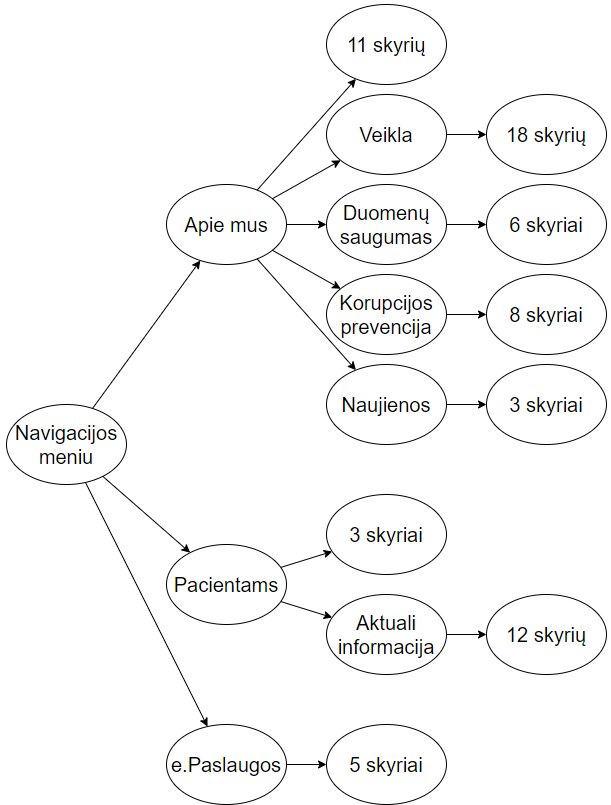
\includegraphics[scale=0.8]{img/NavigacijosMeniuDabartinis}
    \caption{Dabartinio navigacijos meniu diagrama}
    \label{img:NavigacijosMeniuDabartinis}
\end{figure}

Dabartinės sistemos navigacijos meniu pavaizduotas diagramoje (\ref{img:NavigacijosMeniuDabartinis} paveikslas). Šio meniu pirmame lygyje tik trys skyriai, taigi iš šio lygio nedaug galima sužinoti apie tinklapio turinį. Į skyrių „Apie mus“ sudėti 15 skyrių, o 4 iš jų rodo į trečią lygį, iš viso „Apie mus“ skyrius turi 46 vaikinius skyrius, daug daugiau nei bet kuris kitas skyrius. Vienas iš vaikinių skyrių yra nuoroda į paiešką, autoriaus nuomone tai yra perteklinis skyrius, kurio galima atsisakyti, nes paieška matoma visuose puslapiuose. Po pakeitimų gautas navigacijos meniu pavaizduotas \ref{img:NavigacijosMeniuPakeistas} paveiksle.

Atlikti pakeitimai navigacijos meniu:
\begin{enumerate}
	\item Panaikintas trečias lygis perkeliant visus trečio lygio skyrius ir jų tėvinį skyrių vienu lygiu aukštyn
	\item Nauji pirmo lygio skyriai surūšiuoti pagal jų svarbą naudotojai (autoriaus nuomone)
	\item Panaikintas skyrius nurodantis į paiešką
	\item Panaikintas skyriaus „Patalpų nuoma“ duplikatas
	\item Skyriaus „Pacientams“ vaikiniai skyriai apkeisti vietomis su skyriaus „Aktuali informacija“ vaikiniais skyriais
	\item Panaikintas „Apie mus“ skyriaus identiško pavadinimo vaikinis skyrius, kad suvienodinti veikseną tarp skyrių
\end{enumerate}

\begin{figure}[htb]
    \centering
    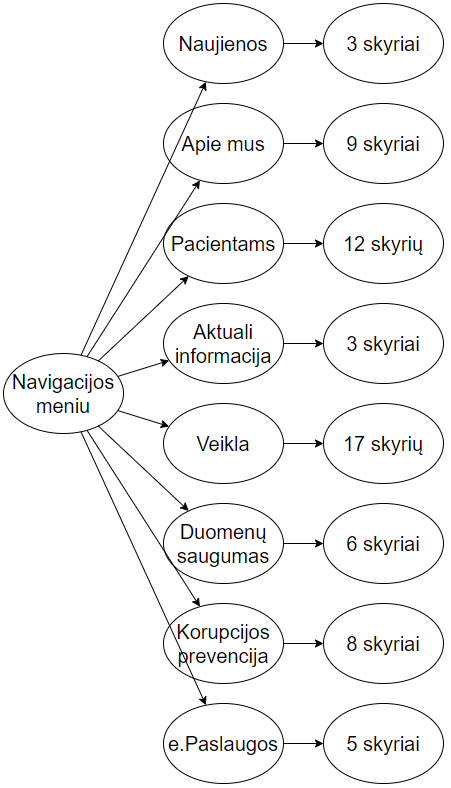
\includegraphics[scale=0.8]{img/NavigacijosMeniuPakeistas}
    \caption{Pakeisto navigacijos meniu diagrama}
    \label{img:NavigacijosMeniuPakeistas}
\end{figure}

\subsection{Sistemos architektūra}
Prieš kuriant tinklapio sistemą reikia apgalvoti, iš kokių dalių ir kaip ji susideda. Tai nuspręsta atsižvelgus į įgyvendinimo sudėtingumą, populiarius sprendimus ir naudotojų poreikius.

Vienas iš populiariausių ir paprasčiausių architektūros modelių yra Modelis-Vaizdas-Valdiklis (Model-View-Controller, toliau MVC)\cite{MVCDefinition}. Šis modelis sudarytas iš trijų sluoksnių: duomenų sluoksnio, vaizdo sluoksnio ir valdiklių sluoksnio. Duomenų sluoksnis atsakingas už duomenis reikalingus programos veikimui, daugeliu atveju duomenų bazę, kurioje gali būti saugomi puslapių tekstai\cite{MVCSO3}. Vaizdo sluoksnis pateikia vartotojui vaizdą, pavyzdžiui puslapį ir mygtukus. Valdiklių sluoksnis skirtas komunikacijai tarp vaizdo ir modelio sluoksnių, jis priima vartotojo įvestį ir pateikia rezultatus iš duomenų bazės. Visa tai leidžia atlikti tinklapiui reikalingas funkcijas kaip duomenų, saugojimas, puslapių rodymas, paieškų atlikimas, filtravimas ir žinučių ar komentarų siuntimas. Naudojant MVC modelį kodas atskiriamas pagal sluoksnius, tai leidžia izoliuoti komponentus ir dėl to kodą lengviau plėsti, kyla mažiau klaidų bei jas lengviau pataisyti. Šios savybės palaiko objektinio programavimo metodiką ir padeda turėti aiškiai suprantamą projekto struktūrą.

Vienas svarbus punktas yra, kad sistema būtų responsyvi ir galėtų aptarnauti didelį kiekį vartotojų, tačiau tai universalus poreikis ir ši architektūra tam netrukdo. Kadangi kuriamas tinklapis neturi išskirtinių bruožų, dėl kurių reikėtų galvoti naujus sprendimus, galima naudoti MVC modelį\cite{MVCSO1, MVCSO2}. Galiausiai, autorius jau turi patirties su šiuo modeliu, taigi nereikės mokytis pagrindų.

\section{Sistemą realizuojančios technologijos}
Norint įgyvendinti sistemą MVC modeliu, reikia pasirinkti kokios technologijos bus naudojamos kiekvienam sluoksniui. Šiuo atveju sluoksnių elementai būtų duomenų bazė ir jos valdymas (Model), puslapiai (View) ir valdikliai (Controller).

\subsection{Technologijos duomenų bazės valdymui}



\subsection{Technologijos puslapių kūrimui}

\subsection{Technologijos valdikliams įgyvendinti}

\sectionnonum{Rezultatai ir išvados}


%Rezultatų ir išvadų dalyje turi būti aiškiai išdėstomi pagrindiniai darbo
%rezultatai (kažkas išanalizuota, kažkas sukurta, kažkas įdiegta) ir pateikiamos
%išvados (daromi nagrinėtų problemų sprendimo metodų palyginimai, teikiamos
%rekomendacijos, akcentuojamos naujovės).


%% PAKEISTAS PAVADINIMAS Į 'Šaltiniai'
\printbibliography[heading=bibintoc, title=Šaltiniai]  % Šaltinių sąraše nurodoma panaudota
% literatūra, kitokie šaltiniai. Abėcėlės tvarka išdėstomi darbe panaudotų
% (cituotų, perfrazuotų ar bent paminėtų) mokslo leidinių, kitokių publikacijų
% bibliografiniai aprašai.  Šaltinių sąrašas spausdinamas iš naujo puslapio.
% Aprašai pateikiami netransliteruoti. Šaltinių sąraše negali būti tokių
% šaltinių, kurie nebuvo paminėti tekste.

% \sectionnonum{Sąvokų apibrėžimai}
%\sectionnonum{Santrumpos}
%Sąvokų apibrėžimai ir santrumpų sąrašas sudaromas tada, kai darbo tekste
%vartojami specialūs paaiškinimo reikalaujantys terminai ir rečiau sutinkamos
%santrumpos.

\appendix  % Priedai
% Prieduose gali būti pateikiama pagalbinė, ypač darbo autoriaus savarankiškai
% parengta, medžiaga. Savarankiški priedai gali būti pateikiami ir
% kompaktiniame diske. Priedai taip pat numeruojami ir vadinami. Darbo tekstas
% su priedais susiejamas nuorodomis.
\sectionnonum{Trys puslapių tipai}

\begin{figure}[H]
    \centering
    
\includegraphics[scale=0.65]{img/Pagrindinis}
    \caption{Pagrindinis puslapis}
    \label{img:PagrindinisPuslapis}
\end{figure}
\begin{figure}[H]
    \centering
    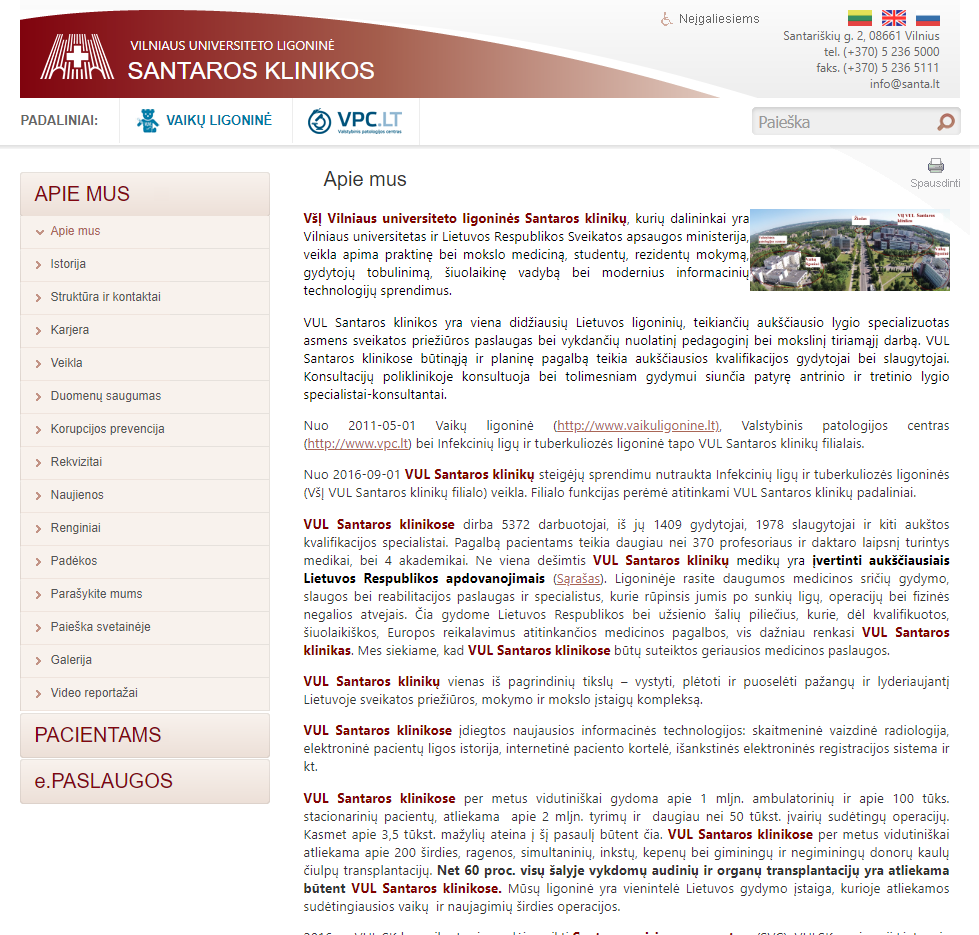
\includegraphics[scale=0.65]{img/Turinys}
    \caption{Turinio puslapis}
    \label{img:TurinysPuslapis}
\end{figure}
\begin{figure}[H]
    \centering
    \includegraphics[scale=0.65]{img/Paieška}
    \caption{Paieškos puslapis}
    \label{img:PaieškaPuslapis}
\end{figure}




%\section{Eksperimentinio palyginimo rezultatai}
% tablesgenerator.com - converts calculators (e.g. excel) tables to LaTeX
%\begin{table}[H]\footnotesize
%  \centering
%  \caption{Lentelės pavyzdys}
%  {\begin{tabular}{|l|c|c|} \hline
%    Algoritmas & $\bar{x}$ & $\sigma^{2}$ \\
%    \hline
%    Algoritmas A  & 1.6335    & 0.5584       \\
%    Algoritmas B  & 1.7395    & 0.5647       \\
%    \hline
%  \end{tabular}}
%  \label{tab:table example}
%\end{table}

\end{document}
